\section{Optimizaciones}

La metodolog\'{i}a utilizada para llevar a cabo las optimizaciones es un
proceso iterativo que incluye los siguientes pasos en cada iteraci\'{o}n:

\begin{itemize}
\item Identificar la parte del c\'{o}digo que consume m\'{a}s tiempo
\item Realizar una optimizaci\'{o}n
\item Comprobar que la optimizaci\'{o}n mejora el rendimiento del programa
\end{itemize}

Utilizando la herramienta \texttt{gprof} se han identificado las partes del
c\'{o}digo original que consumen la mayor\'{i}a del tiempo de ejecuci\'{o}n.
La salida proporcionada por dicha herramienta es la siguiente:


En consecuencia, el objetivo de la primera optimizaci\'{o}n es la funci\'{o}n
\texttt{electric\_field}.

\subsection{Opt1: Evitar llamadas a gaddress}

La funci\'{o}n \texttt{gaddress} se encarga de calcular un indice de un
vector a partir de los cuatro par\'{a}metros que recibe. En el c\'{o}digo de
\texttt{electric\_field} se llama a la funci\'{o}n \texttt{gaddress} en
muchas ocasiones de forma innecesaria. La llamada es innecesaria porque la
secuencia de valores de retorno que generan las llamadas a \texttt{gaddress}
en el c\'{o}digo original es 0, 1, 2, ..., grid\_size-1, grid\_size+2,
grid\_size+3, etc. El c\'{o}digo original es el siguiente:

\begin{lstlisting}[]
for( x = 0 ; x < grid_size ; x ++ ) {
  for( y = 0 ; y < grid_size ; y ++ ) {
    for( z = 0 ; z < grid_size ; z ++ ) {
      grid[gaddress(x,y,z,grid_size)] = ...
    }
  }
}
\end{lstlisting}

La optimizaci\'{o}n propuesta consiste en cambiar la llamada a
\texttt{gaddress} por un simple contador que se incrementa en uno en cada
iteraci\'{o}n sobre \texttt{z} y en dos en cada iteraci\'{o}n sobre
\texttt{y}, generando as\'{i} los \'{i}ndices correctamente. El c\'{o}digo
resultante es el siguiente:

\begin{lstlisting}[]
i = 0;
for( x = 0 ; x < grid_size ; x ++ ) {
  for( y = 0 ; y < grid_size ; y ++ ) {
    for( z = 0 ; z < grid_size ; z ++ ) {
      grid[i] = ...
      i++;
    }
    i += 2;
  }
}
\end{lstlisting}

Esta optimizaci\'{o}n se puede aplicar de la misma forma en otros puntos, como
en \texttt{electric\_field\_zero\_core} o en el primer bucle de
\texttt{electric\_point\_charge}.

\subsection{Opt2: Evitar saltos}

\subsection{Opt3: Evitar operaciones de coma flotante}

\subsection{Opt4: Evitar llamadas a sistema}

\subsection{Opt5: Unrolling}

\subsection{Opt6: Vectorizaci\'{o}n}

\subsection{Ayuda}

Peque\~{n}a ayuda (mirar optimizaciones.tex para ver el c\'{o}digo):

Como poner una lista de elementos:
\begin{itemize}
   \item Elemento 1
   \item Elemento 2
\end{itemize}

Como poner una figura:
\begin{figure}[ht]
   \centering
   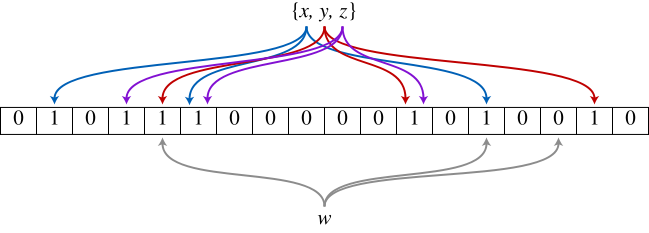
\includegraphics[keepaspectratio=true,width=.6\textwidth]{figures/muestra}
\end{figure}

Como poner una tabla:
\begin{center}
   \begin{tabular}{| c || c | c | c |}
      \hline
      	           & Load	& Store		& Total		\\ \hline \hline
	Accesses   & 105353	& 21423		& 126776	\\ \hline
	Hits       &  11644	&  1837		&  13481	\\ \hline
	Misses     &  93709 	& 19586		& 113295	\\ \hline
	Miss rate  & 88.95\%	& 91.43\%	& 89.37\%	\\ \hline
   \end{tabular}
\end{center}

Como poner c\'{o}digo:

\begin{lstlisting}[]
for( x = 0 ; x < grid_size ; x ++ ) {
  for( y = 0 ; y < grid_size ; y ++ ) {
    for( z = 0 ; z < grid_size ; z ++ ) {
      grid[gaddress(x,y,z,grid_size)] = ...
    }
  }
}
\end{lstlisting}

% vim: filetype=tex tw=75
